% $Author: ducasse $
% $Date: 2005/05/16 13:38:08 $
% $Revision: 1.1.1.1 $
\ifx\wholebook\relax\else
\documentclass{report}
\usepackage{times}
\usepackage{epsfig}
\usepackage{alltt}
\usepackage{xspace}
\usepackage{graphicx}
\usepackage{ifpdf}
\usepackage{ifthen}
\usepackage{amsmath}
\usepackage{a4wide}

\graphicspath{{figures/}} 

\ifpdf
\DeclareGraphicsExtensions{.pdf, .jpg, .tif, .png}
\else
\DeclareGraphicsExtensions{.eps, .jpg}
\fi

\newboolean{toseecomment}
\setboolean{toseecomment}{false}
%%change to false to hidde comment 
\newcommand{\comment}[1]{\ifthenelse{\boolean{toseecomment}}{$\blacktriangleright$ \textit{#1}$\blacktriangleleft$}{}}

\newcommand{\commented}[1]{}

\newboolean{seevwspecific}
\setboolean{seevwspecific}{true}
\newcommand{\vwspecific}[1]{\ifthenelse{\boolean{seevwspecific}}{#1}{}}

\newboolean{seecategoryspecific}
\setboolean{seecategoryspecific}{false}
\newcommand{\categoryspecific}[1]{\ifthenelse{\boolean{seecategoryspecific}}{#1}{}}

\newboolean{seestorespecific}
\setboolean{seestorespecific}{true}
\newcommand{\storespecific}[1]{\ifthenelse{\boolean{seestorespecific}}{#1}{}}

\newboolean{seesqueakspecific}
\setboolean{seesqueakspecific}{false}
\newcommand{\squeakspecific}[1]{\ifthenelse{\boolean{seesqueakspecific}}{#1}{}}


\newcommand{\category}[0]
{\ifthenelse{\boolean{seestorespecific}}
	{package\xspace}
	{category\xspace}}

\newcommand{\ct}[1]{\texttt{#1}\xspace}
\newcommand{\stc}[1]{{\small {\sf #1}}\xspace}
\newcommand{\ST}{{\textsc Smalltalk}\xspace}
\newcommand{\tab}{\makebox[4em]{}}
\newcommand{\ttt}[1]{{\tt #1}}
\newcommand{\chev}{\ttt{>>}}
\newcommand{\vw}{VisualWorks\xspace}
\newcommand{\sq}{Squeak\xspace}
\newcommand{\store}{Store\xspace}
\renewcommand{\chaptername}{Exercise}
\newcommand{\exercise}{\vspace{0.2cm}\noindent \textbf{Exercise:}\xspace}

\newsavebox{\fminibox}
\newlength{\fminilength}

% Fait un truc encadre
\newenvironment{fminipage}[1][\linewidth]
  {\setlength{\fminilength}{#1-2\fboxsep-2\fboxrule}
        \begin{lrbox}{\fminibox}\begin{minipage}{\fminilength}}
  { \end{minipage}\end{lrbox}\noindent\fbox{\usebox{\fminibox}}}

% Pareil mais pas encadre (a utiliser pour ne pas couper une fonction

\newenvironment{nminipage}[1][\linewidth]
  {\setlength{\fminilength}{#1}
        \begin{lrbox}{\fminibox}\begin{minipage}{\fminilength}}
  { \end{minipage}\end{lrbox}\noindent\mbox{\usebox{\fminibox}}}

% Un alltt encadre
\newenvironment{falltt}
  {\vspace*{0.3cm}\begin{fminipage}\begin{alltt}}
  {\end{alltt}\end{fminipage}\vspace*{0.3cm}}

% Un alltt pas encadre
\newenvironment{nalltt}
  {\vspace*{0.3cm}\begin{nminipage}\begin{alltt}}
  {\end{alltt}\end{nminipage}\vspace*{0.3cm}}

% Une fonction encadree
\newenvironment{ffonction}[1]
  {\begin{fonction}[#1]
        \begin{fminipage}
\begin{alltt}
\rule{\linewidth}{0.5pt}}
{\end{alltt}\end{fminipage}\end{fonction}}

\newenvironment{codeonepage}
  {\begin{nminipage}\vspace*{0.2cm}\hrule\vspace*{0.1cm}
\begin{alltt}}
  {\end{alltt} \vspace*{-0.2cm}\hrule \vspace*{0.2cm} \end{nminipage}}

\newenvironment{code}
  {\vspace*{0.1cm}\hrule\vspace*{-0.1cm}\begin{alltt}}
  {\end{alltt}\vspace*{-0.2cm}\hrule \vspace*{0.1cm}}


\begin{document}
\fi

\chapter{Seaside Tutorial}

\mainauthor{lukas renggli}

% extra packages
%\usepackage{amssymb}
%\parskip 1ex


% S E T T I N G S
% % % % % % % % % % % % % % % % % % % % % % % % % % % % % % % % % % % % %
%\title{Tutorial\\
%Seaside Web Applications}
%\author{Lukas Renggli\\
%\texttt{renggli@iam.unibe.ch}\\
%\texttt{www.lukas-renggli.ch}\\
%\\
%Software Composition Group\\
%Institut f\"ur Informatik und angewandte Mathematik\\
%Universit\"at Bern, Switzerland\\
%\\
%netstyle.ch GmbH\\
%Bern, Switzerland}
%\date{February 2005}

%
% D O C U M E N T   S T A R T
% % % % % % % % % % % % % % % % % % % % % % % % % % % % % % % % % % % % %
%\begin{document}

% title
%\maketitle
%\newpage

% table of conents
%\tableofcontents
%\newpage


% G E T T I N G   S T A R T E D
% % % % % % % % % % % % % % % % % % % % % % % % % % % % % % % % % % % % %
\section{Getting Started}

Follow the instructions given on the slides to install Seaside. Make sure your Seaside server is up and running by accessing the example application at \ct{http://\-localhost:8080/\-seaside/\-counter} in Squeak or at \ct{http://\-localhost:8008/\-seaside/\-go/\-counter} in VisualWorks.

In Squeak load the monticello package \ct{tutorial.mcz} and in VisualWorks the parcel \ct{tutorial.pcl}. Both packages contain examples shown during the presentation and some class skeletons that will assist you to do these exercises.

Save your image. From now on work within a copy of this image, so that you can easy go back to a working configuration, in case you severely screw something up.


% D E V E L O P M E N T   T O O L S
% % % % % % % % % % % % % % % % % % % % % % % % % % % % % % % % % % % % %
\section{Development Tools}

\exercise{Use your web browser to navigate to the counter example application. Toggle on the halos to see the border of the component this application is built of. Experiment and interact with the application in render- and source-mode.}

\exercise{Change the behaviour of the increase and decrease buttons: edit the methods \method{increase} and \method{decrease} from within the web browser to increase by \ct{2} and decrese by \ct{3}.}

\exercise{Inspect the living component from within the web browser. There are two instance variables visible, whereas \ct{count} is representing the state of the component. The other instance variable is defined in a super-class of \class{WACounter} and will be discussed later on.}

\exercise{Change the background color of the web application by using the style editor from within your web browser. Try using something like \ct{body \{ background-color: yellow; \}}.}

\question{Why do you think the style editor is used more often in industrial settings than the system browser?}

\exercise{Introduce an error to the method \method{increase} using your web browser. Play with your application so that the error occurs. Click on the \emph{debug} link which opens a debugger within your image. Fix the bug and proceed the evaluation.}


% C O N T R O L   F L O W
% % % % % % % % % % % % % % % % % % % % % % % % % % % % % % % % % % % % %
\section{Control Flow}

During the theoretical part an example was shown where the user had to guess a number the computer was thinking of. In this exercise we will have a look at the implementation of two similar games. Some skeletons are provided, so you don't need to implement all by yourself.


\subsection{User Guesses a Number}

\exercise{Have a look at the source code of \class{STUser\-Number\-Guesser} in the package \package{Tutorial-Flow} and play the game several times to make sure it works as expected.}

\exercise{Modify the method \method{go} in \class{STUser\-Number\-Guesser} to count the number of guesses. Show the total number of guesses the user required to get the right number in the end of the game.}

\question{Try using the back button while playing the game. How does the application handle this?}

\question{What happens if you open multiple windows in the same session and play within the different windows independently?}

\questionstar{Is it possible to cheat the counter by using the back button or by opening new windows within the same session? Does this behavior change if you use an instance variable instead of a temporary one for counting?}


\subsection{Computer Guesses a Number}

\exercise{Write a new web application that allows the computer to guess a number the user is thinking of. In case you run into troubles, you can always have a look at the implementation of \class{STUser\-Number\-Guesser}.}

\begin{enumerate}
\item Create a subclass of \class{WATask} called \class{STComputer\-Number\-Guesser}.
\item Create an initialization method on the class side of the newly created class, registering the component as a new web application with the path segment \ct{cng}.
\item Implement the method \method{go} following the rules of the game. Use \method{inform:} to tell the user what he should do and \method{confirm:} to ask the user if the guess of the computer is too big.
\item Play the game several times to make sure it works as expected.
\end{enumerate}

\exercise{Implement yet another task asking the user if he wants to guess or not. Depending on the answer either call \class{STUser\-Number\-Guesser} or \class{STComputer\-Number\-Guesser}. Modify those two classes to answer the numbers of steps required and call them from within your new task. Don't forget to register your new application with a class initialization method.}


\subsection{TicTacToe Game}

There are three prepared classes for this game in the package \package{Tutorial-TicTacToe} following the \emph{MVC-Pattern}:

\begin{description}
\item[Model] \class{STTicTacToeController} is a simple model of a game holding the current board configuration. It includes methods to access and modify its configuration (\method{boardAt:} and \method{boardAt:put:}) and to call an algorithm in order to look for the best possible move of a given player (\method{find:}).
\item[View] \class{STTicTacToeView} is a simple Seaside view onto the game model. You will learn later on how to create views with Seaside.
\item[Controller] \class{STTicTacToeController} is a subclass of \class{WATask} and this is the place that needs your work now. It already implements a few convenience methods like \method{newModel}, \method{computerMove} and \method{userMove}.
\end{description}

\exercise{Register \class{STTicTacToeController} as a new web-application, but this time don't use a class initialization method but the configuration interface. Make sure that you have a method \method{canBeRoot} on the class-side so that Seaside recognizes this class as a possible root of a web application. Browse to \ct{http://\-localhost:8080/\-seaside/\-config} when using Squeak or \ct{http://\-localhost:8008/\-seaside/\-go/\-config} when using VisualWorks, enter your password, add a new entry point with the name \ct{ttt} and select \class{STTic\-Tac\-Toe\-Controller} as the root component.}

\exercise{Implement the game in the method \method{go} using the provided convenience methods. You will also need some testing methods of the model to check if the game is finished (\method{isFinished}) and who was the winner (\method{winner}). Don't put all your code into one single method, split it among different ones to ensure readability. Ask the user in the beginning of the game if he prefers to start playing or not.}

\exercisestar{Ensure that the user can't cheat the game by using the back button of the web browser. Don't wrap too much or to few of your code into \method{isolate:} blocks.}


% C O M P O N E N T S
% % % % % % % % % % % % % % % % % % % % % % % % % % % % % % % % % % % % %
\section{Components}

For the rest of this tutorial we will be working on an example of a possible real-world web application: it should be useable by a theater having different plays in its program. The application should manage the plays, the shows and the booking of the tickets.


\subsection{Introduction}
Here we will be starting step by step building up this project. Follow the exercises one by one as they depend on each other. However don't let you hinder from bringing in your own ideas and from implementing some extra features, if you think they could be useful for this project.

\begin{figure}[htbp]
\begin{center}
	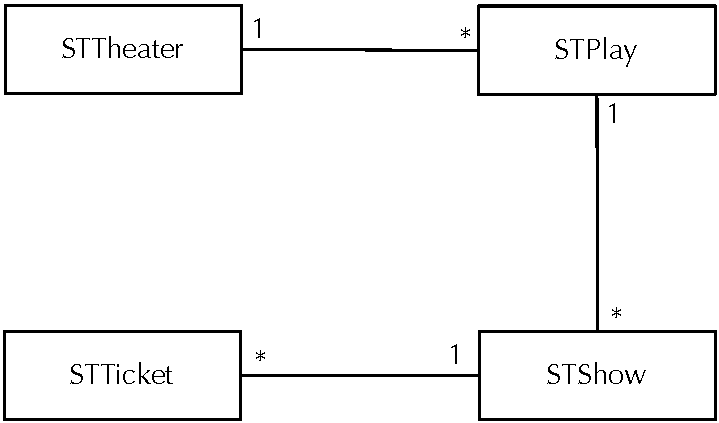
\includegraphics[scale=0.6]{theater-model}
	\caption{Theater-Model}
	\label{theater-model}
\end{center}
\end{figure}

All the code altogether should be put into the bundle \bundle{Tutorial-Theater} that contains some packages, namely \package{Theater-Model}, \package{Theater-View} and \package{Theater-Tests}. The package \package{Theater-Model} contains a very simple model, as seen in \figref{theater-model}, to be used to build up a web-interface around. Feel free to enhance the model when you need to do so, but do run the tests and add new ones to make sure that all the features work as expected after your modifictions.

On the class side of \class{STTheater} you can find a method \method{default} returning the domain model to be used for the web application. Usually you do not keep your model just within the image, but use a proper external storage mechanism instead: this can be simply done by dumping out the object graph to the filesystem from time to time or by using a relational- or object-database. However, as possible storage strategies are out of the scope here, we will just keep everything within the image.

\begin{figure}[htbp]
\begin{center}
	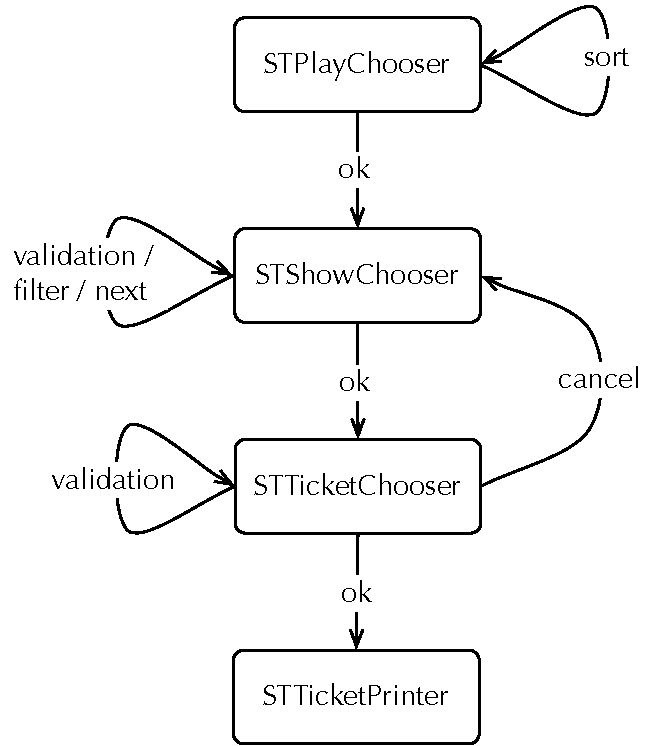
\includegraphics[scale=0.6]{theater-flow}
	\caption{Theater-Flow as defined by \class{STBuyTicketTask}}
	\label{theater-flow}
\end{center}
\end{figure}

\exercise{Start out by creating a new task called \class{STBuyTicketTask} that will model the steps required to buy a ticket. Register it as a new Seaside application as you will need it later on to test your components. Leave the method \method{go} empty for now. This method should define the flow as seen in \figref{theater-flow} by the end of the tutorial.}


\subsection{Choosing a Play}

\begin{figure}[htbp]
\begin{center}
	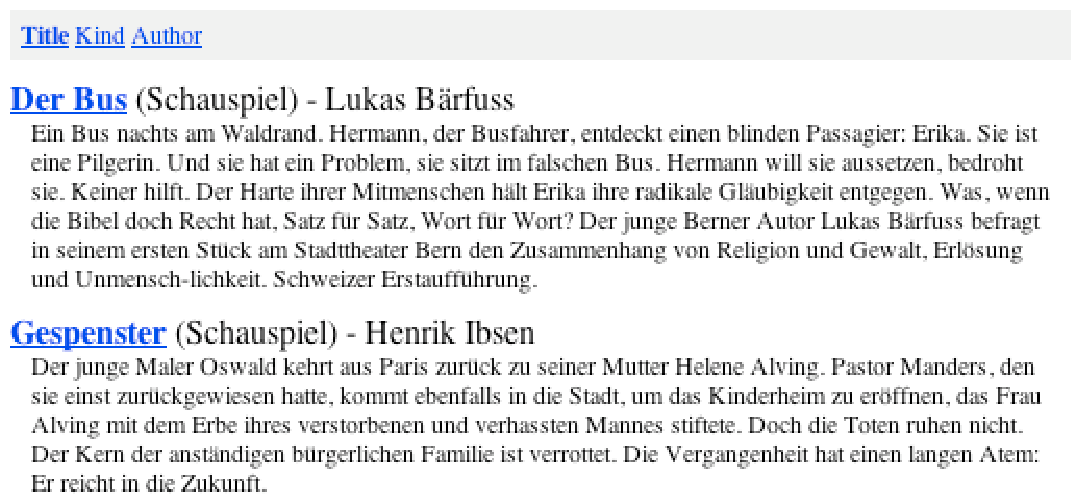
\includegraphics[scale=0.5]{theater-playchooser}
	\caption{View of \class{STPlayChooser}}
	\label{theater-playchooser}
\end{center}
\end{figure}

\exercise{Create a subclass of \class{WAComponent} called \class{STPlayChooser} that will give the user the possibility to choose a theater-play. Add an instance variable \ct{plays} and create accessors to hold a collection of plays that should be displayed with this component. Call your newly created component from \class{STBuyTicketTask}, but don't forget to initialize it with the collection of plays. If you browse to your application, you should get a blank page as you haven't defined any view yet.}

\begin{figure}[htbp]
\begin{center}
	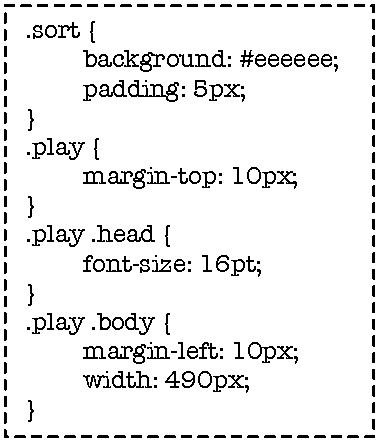
\includegraphics[scale=0.5]{theater-playchooserstyle}
	\caption{Stylesheet of \class{STPlayChooser}}
	\label{theater-playchooserstyle}
\end{center}
\end{figure}

\exercise{Implement the method \method{renderContentOn:}. As a first step, enumerate the plays and display the title of each. If you go back to your web browser and refresh, you should see the titles now. Then display the other information you get from the model. Use your own style sheet or copy the example from \figref{theater-playchooserstyle} to make the output look like \figref{theater-playchooser}.}

\exercise{So far there is no interaction possible with the component. Create an anchor-callback \method{anchorWithAction:do:} around the title and answer the selected play to the caller. Test your code by extending the task that is calling your component and inform the user about the selected play.}

\exercisestar{To set up the list of the plays more convenient, add three links at the top of the page to make it possible to sort the plays according to \method{title}, \method{kind} or \method{author}. To remember the state of the selected sort order you need to add another instance variable. Make it also possible to sort in reverse order by clicking a second time onto the same link.}


\subsection{Choosing a Show}

\exercise{Create another subclass of \class{WAComponent} called \class{STShowChooser} that allows the user to choose a show. Add instance variables to hold a collection of shows to choose from and one for the current selection. Create appropriate accessors and call your newly created and properly initialized component from \class{STBuyTicketTask}.}

\begin{figure}[htbp]
\begin{center}
	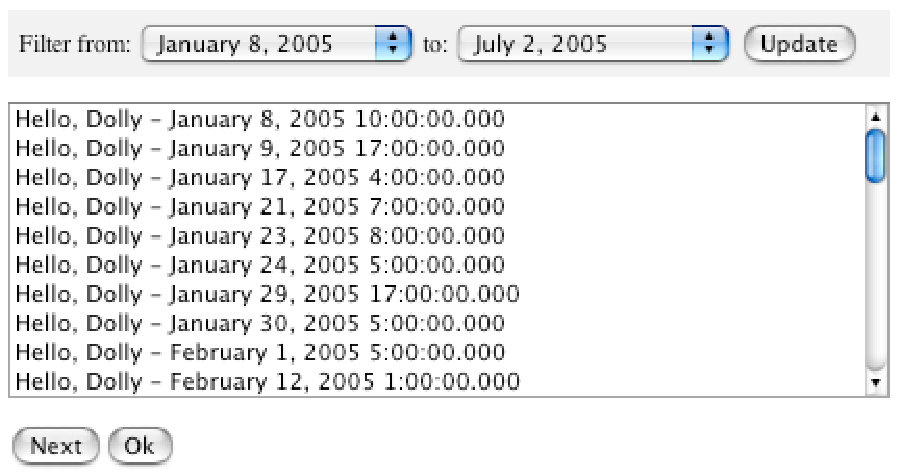
\includegraphics[scale=0.5]{theater-showchooser}
	\caption{View of \class{STShowChooser}}
	\label{theater-showchooser}
\end{center}
\end{figure}

\exercise{Implement the method \method{renderContentOn:} using \figref{theater-showchooser} as a reference; don't worry about the filter yet. Make sure hitting \emph{ok} only answers if the user actually selected a valid show, else show a message that a selection is missing and return to the dialog. Add a button to select the next possible show automatically.}

\exercisestar{Implement a facility to allow filtering for a certain date range. Write a method returning a possible list of dates and add two instance variables to keep the selected date for start and end of the period to be filtered. Render two drop-down boxes and a button to update the filtered list. Use live-callbacks to update the list of shows without the need to press the update button anymore.}

\exercisestar{Experiment with other form controls. How does the interface look like when using option-boxes instead of the list? What do you need to change in the code?}


\subsection{Buying and Printing Tickets}

\exercise{Write a component that allows the user to select the number of tickets he wants to buy. Give an error message, if there are not enough places available for the selected show or if the user doesn't enter a valid number. Update the domain model according to the tickets sold and answer a collection of tickets to the task. The view of a minimal implementation can be seen in \figref{theater-ticketchooser}.}

\begin{figure}[htbp]
\begin{center}
	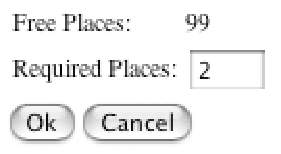
\includegraphics[scale=0.5]{theater-ticketchooser}
	\caption{View of \class{STTicketChooser}}
	\label{theater-ticketchooser}
\end{center}
\end{figure}

\exercise{Last but not least write yet another component printing out a collection of tickets. This might look like \figref{theater-ticketprinter}. No links or form elements are required in this component. Update your flow accordingly.}

\begin{figure}[htbp]
\begin{center}
	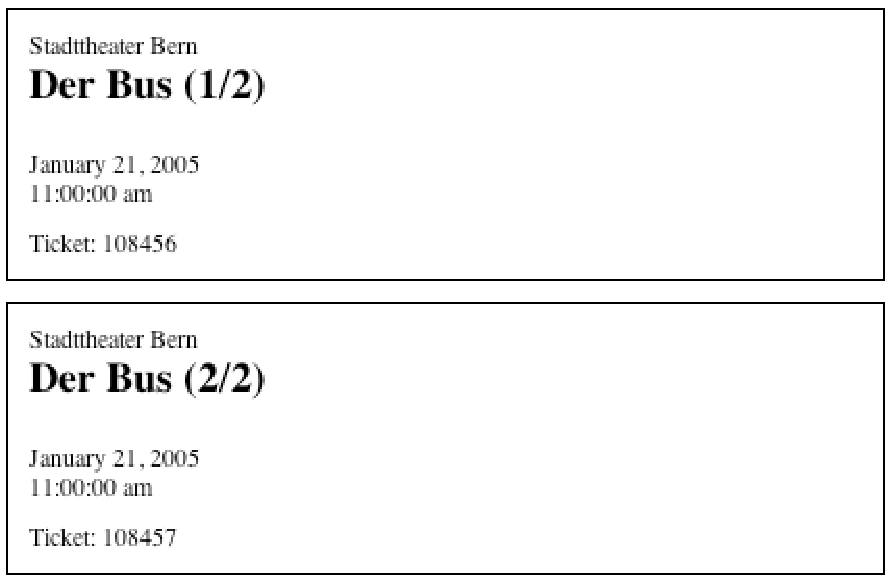
\includegraphics[scale=0.5]{theater-ticketprinter}
	\caption{View of \class{STTicketPrinter}}
	\label{theater-ticketprinter}
\end{center}
\end{figure}

\exercise{Make sure that your application implements all the paths that are visible in the state diagram in \figref{theater-flow}. Make sure that the user cannot go back after having bought the tickets.}


% C O M P O S I T I O N
% % % % % % % % % % % % % % % % % % % % % % % % % % % % % % % % % % % % %
\section{Composition}

In this section we will compose different components we have written before. Create a few more components and plug together an appealing and simple user interface.

\begin{figure}[htbp]
\begin{center}
	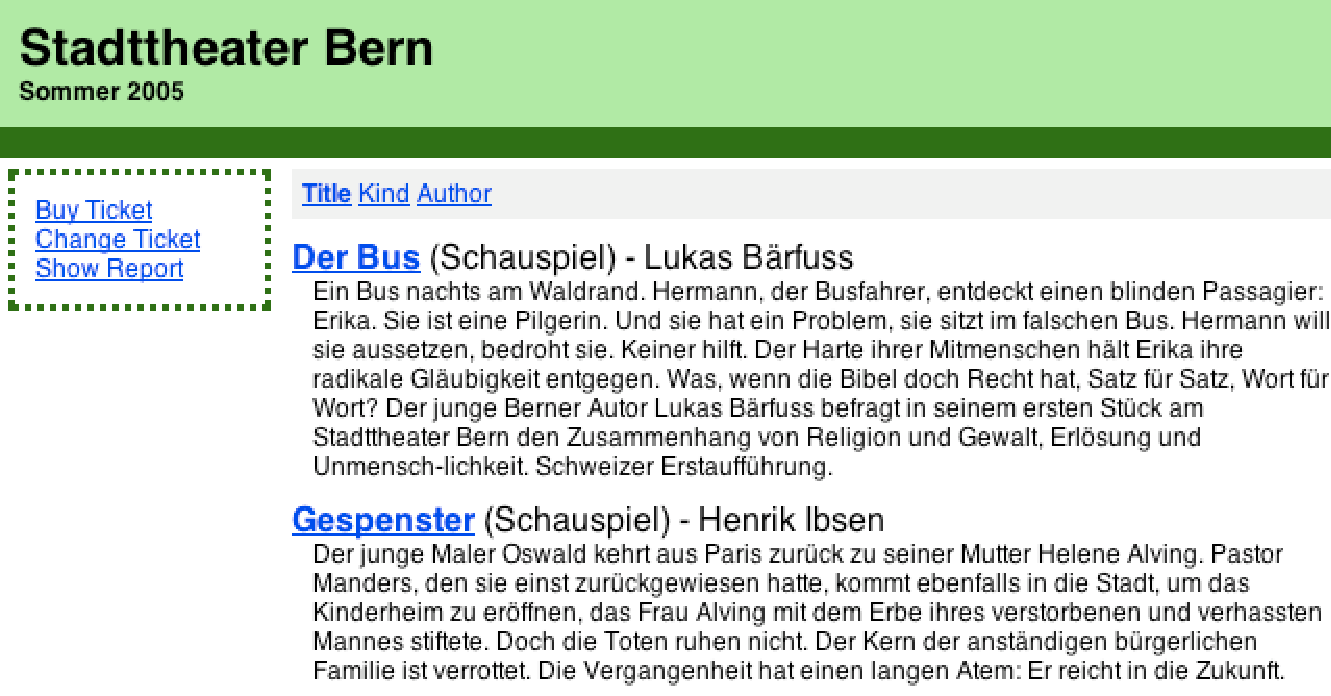
\includegraphics[scale=0.5]{theater-mainframe}
	\caption{View of \class{STMainFrame}}
	\label{theater-mainframe}
\end{center}
\end{figure}


\subsection{Frame, Subcomponent and Backtracking}

\exercise{Create a new subclass of \class{WAComponent} and register it as a new entry point to your application. Render into different div-tags the name of the theater and the current season; you can find this information in the model. Also create a simple menu that is empty for now. Create a style-sheet to make the application look nicer.}

\exercise{Add an instance variable to your main-frame to hold a child component. Create a method \method{buyTicket} that initializes the variable with a new instance of \class{STBuyTicketTask} and send \method{buyTicket} in the initialization method of the component. Place the child beside the menu you have created before. Don't forget to implement the message \method{children}, else you will sooner or later run into troubles. Create a menu item called \emph{Buy Ticket} that sends the message \method{buyTicket} when clicked. Enjoy the application with the halos turned on.}

\exercisestar{Test the new functionality you implemented. Especially try out the behavior of the application when using the back-button. Try clicking on \emph{Buy Ticket}, hit the back-button of your web-browser and then click on any link or control within the child-component. Why do you get an error? Fix the problem and make sure everything works as expected.}


\subsection{Reuse of Components}

In this part of the exercises you are basically free about the implementation details of a new requirement of the application: The theater company wants to be able to let the customers return tickets and exchange them with another one from the same play but a different show.

\exercise{Use the id of the ticket to identify the one to be replaced. Probably you need to improve the model to make the necessary mutations possible. Also write tests to ensure it works as expected. For the web interface try to write as few lines of code as possible. Reuse the existing components that you have written in the previous steps. You might also want to use components provided by the framework. The example solution requires 7 lines of code, including the validation of the ticket id. Can you do it with less lines of code?}


\subsection{Reporting and Batching}

\exercise{Create a new component called \class{STShowReport} showing a report of all the shows from the model as seen in \figref{theater-showreport}. Use \class{WABatchedList} to enable the batching of the huge list and only display 10 items at once. For the reporting you might want to use \class{WATableReport} or write your own component. By default the list should be sorted according to the timestamp. Add the new component to the menu in the main-frame.}

\begin{figure}[htbp]
\begin{center}
	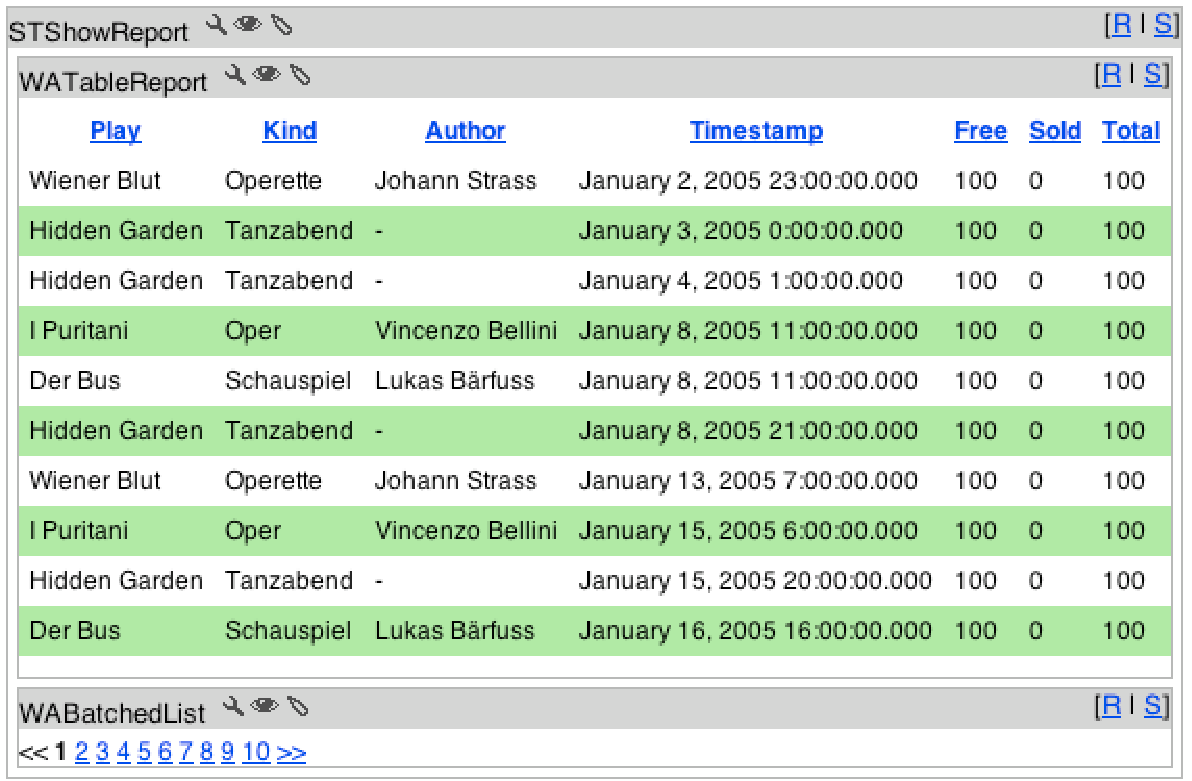
\includegraphics[scale=0.5]{theater-showreport}
	\caption{View of \class{STShowReport} with halos toggled on}
	\label{theater-showreport}
\end{center}
\end{figure}


\subsection{Editing a Play}

In this part we are going to implement a dialog to edit the attributes of a play. Have a look at \figref{theater-editplay} to get an idea of the look. Add a link to the title of every play in your report that calls the component you are going to create in the following exercise:

\exercise{Create a new subclass of \class{WAComponent} and add an instance variable to hold the play. In the method \method{initialize} wrap the component with two decorations: 

\begin{enumerate}
	\item \class{WAFromDecoration} to render a form around the component and display \emph{ok} and \emph{cancel} buttons.
	\item \class{WAValidationDecoration} to validate the input fields and display an error message if necessary.
\end{enumerate}

Ensure that the validation errors are properly displayed and that the model isn't touched when hitting cancel.}

\begin{figure}[htbp]
\begin{center}
	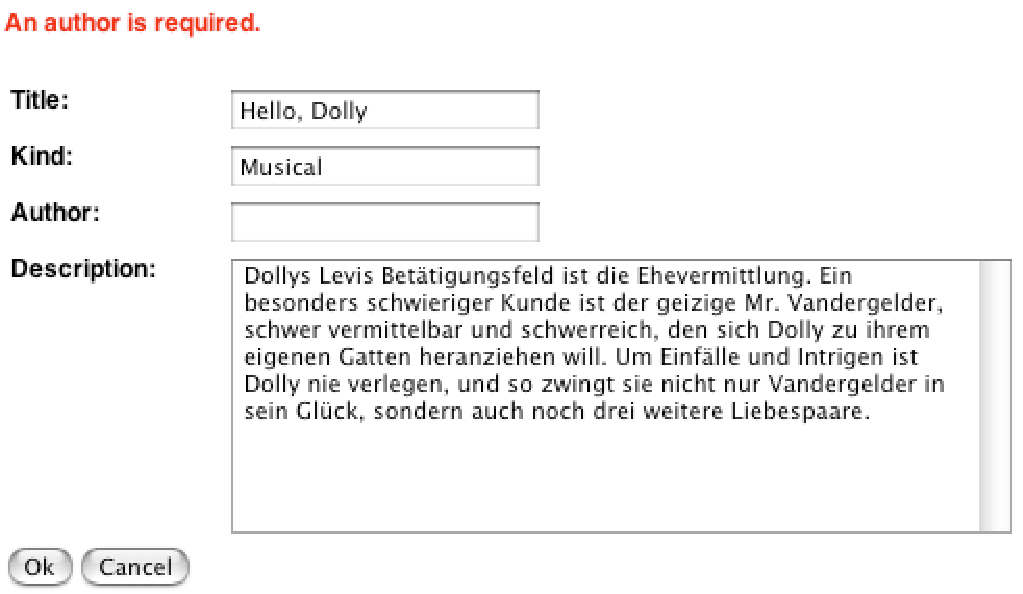
\includegraphics[scale=0.5]{theater-editplay}
	\caption{View of \class{STEditPlay}}
	\label{theater-editplay}
\end{center}
\end{figure}

\exercisestar{Load Mewa and try to write the same dialog using a descriptive meta model.}


% A D V A N C E D
% % % % % % % % % % % % % % % % % % % % % % % % % % % % % % % % % % % % %
\section{Advanced}

\subsection{Continuations}

To answer the following question it might be useful to have a look at the class \class{Continuation}. You might also want to run the different tests of \class{Continuation\-Test} and type and evaluate a few expressions in the workspace.

\question{When should one \emph{not} use a continuation based web framework?}

\question{How are continuations implemented in Smalltalk? Why are there no primitives required?}

\question{What about the time- and space-performance of continuations?}

\questionstar{Why is the implementation of the class \class{Continuation} polymorphic to \class{BlockClosure}? What are the differences?}

\questionstar{When are ensure-blocks evaluated, if you create a continuation within a protected context?}

\subsection{Bookmark-able URLs}

\exercise{Implement \method{updateUrl:} in the three top-level sub-components of your web application and add an appropriate path-element to the URL. Depending on the context of your application, the URL should now look like: \ct{../theater/buy}, \ct{../theater/change} and \ct{../theater/report}.}

\exercise{So far it isn't possible to navigate to these sub-components directly using an URL. To get the desired result, create a subclass of \class{WARender\-Loop\-Main} called \class{STRenderLoopMain} and override the message \method{start:} to parse the URL and to setup the root component as requested.}


% A P P E N D I X
% % % % % % % % % % % % % % % % % % % % % % % % % % % % % % % % % % % % %
%\section*{Appendix}
%
%\subsection*{Creative Commons License -- Attribution-ShareAlike}
%
%This is a human-readable summary of the Legal Code (the full license) available at \ct{http://creativecommons.org/\-licenses/\-by-sa/\-2.0/\-legalcode}.

%\paragraph{You are free:}
%\begin{itemize}
%	\item to copy, distribute, display, and perform the work	
%	\item to make derivative works
%	\item to make commercial use of the work
%\end{itemize}

%\paragraph{Under the following conditions:}
%\begin{itemize}
%	\item Attribution. You must give the original author credit.
%	\item Share Alike. If you alter, transform, or build upon this work, you may distribute the resulting work only under a license identical to this one.
%\end{itemize}

%\begin{itemize}
%	\item For any reuse or distribution, you must make clear to others the license terms of this work.
%	\item Any of these conditions can be waived if you get permission from the copyright holder.
%\end{itemize}



\ifx\wholebook\relax\else\end{document}\fi